\section{Fast Compression in Practice}
\label{sec:results}

Despite the near-linear time algorithm described in Sections~\ref{sec:theory_0} and~\ref{sec:theory}, the coreset construction of \cref{alg:main} nonetheless
requires a bounded approximation to the original task before the sampling can occur. Although theoretically justified, it is unclear how necessary this is in
practice -- would a worse approximation factor still be representative of the dataset for practical purposes? We answer this question by defining a suite of
algorithms, datasets and evaluation procedures that allow for a comprehensive study of speed vs. accuracy tradeoffs in compression for clustering.  We begin by
describing our experimental setup before showing results in both the static and streaming settings. We note that these results correspond directly to
downstream clustering tasks. Unless stated otherwise, our experimental results focus on the $k$-means task.

\subsection{Experimental Setup}
\paragraph*{Metrics}
\label{sssec:metrics}

We analyze the sampling methods along two metrics -- compression accuracy and construction time. Although measuring runtime is standard, it is unclear how to
confirm that a subset of points satisfies the coreset property over all solutions. To this end, we use the distortion measure introduced in~\cite{chrisESA} $
\max \left( \dfrac{\cost(P, \calC_{\Omega})}{\cost(\Omega, \calC_{\Omega})}, \dfrac{\cost(\Omega, \calC_{\Omega})}{\cost(P, \calC_{\Omega})} \right),$ where
$\calC_{\Omega}$ is a candidate solution computed over the coreset $\Omega$. This will be within $1+\varepsilon$ if the coreset guarantee is satisfied
but may be unbounded otherwise.  We refer to this as the \emph{coreset distortion}.

\begin{table}
    \centering
    \begin{tabular}{lrr}
        Dataset & Points & Dim \\
        \hline
        \emph{Adult} & 48\,842 & 14 \\
        \emph{MNIST} & 60\,000 & 784 \\
        \emph{Song} & 515\,345 & 90 \\
        \emph{Cover Type} & 581\,012 & 54 \\
        \emph{Census} & 2\,458\,285 & 68 \\
        \hline
    \end{tabular}
    \caption{Description of real world datasets}
    \label{tbl:datasets}
\end{table}


\paragraph*{Algorithms}
\label{ssec:algorithms}

We compare Fast-Coresets (Algorithm~\ref{alg:main}) against 5 different benchmark sampling strategies that span the space between optimal time and optimal
accuracy.
\begin{description}
        \item \emph{- Standard uniform sampling}. Each point is sampled with equal probability and weights are set to $n / m$, where $m$ is the size of the sample.
        \item \emph{- Standard sensitivity sampling \cite{LS10}}. We refer to Section~\ref{sec:preliminaries}.
        \item \emph{- Lightweight coresets \cite{bachem2018scalable}}. Obtain a coreset by sampling sensitivity values with respect to the $1$-means solution,
            i.e. sensitivities are given by $\hat{s}(p) = 1/|P| + \cost(p, \mu) / \cost(P, \mu)$, where $\mu$ is the dataset mean.
        \item \emph{- Welterweight coresets}. For any $j \in \{1,..., k\}$, we compute a coreset using sensitivity sampling with respect to a candidate
            $j$-means solution.
        \item \emph{- BICO \cite{bico}}. Utilizes BIRCH \cite{birch} to produce a $k$-means coreset in a stream.
\end{description}

\begin{table*}
    \centering
    \vspace*{-0.1cm}
    \tiny
    \begin{tabular}{|c|cc|cc|cc|cc|}
        \hline
        & \multicolumn{8}{c|}{Method} \\
        \cline{2-9} & \multicolumn{2}{c|}{Uniform Sampling} & \multicolumn{2}{c|}{Lightweight} & \multicolumn{2}{c|}{Welterweight} & \multicolumn{2}{c|}{Fast Coreset} \\
        & $m=40k$ & $m=80k$ & $m=40k$ & $m=80k$ & $m=40k$ & $m=80k$ & $m=40k$ & $m=80k$ \\
        \cline{2-9}
        $c$-outlier & 405 $\pm$ 24K & 159 $\pm$ 20K & 1.07 $\pm$ 0.0 & 5.63 $\pm$ 84.6 & 9.44 $\pm$ 105 & 1.03 $\pm$ 0.0 & 1.12 $\pm$ 0.0 & 1.05 $\pm$ 0.0 \\
        Geometric & 86.3 $\pm$ 8.4K & 21.8 $\pm$ 652 & 1.05 $\pm$ 0.0 & 11.6 $\pm$ 452 & 1.11 $\pm$ 0.0 & 1.03 $\pm$ 0.0 & 1.11 $\pm$ 0.0 & 1.05 $\pm$ 0.0 \\
        Gaussian Mix. & 3.17 $\pm$ 3.42 & 1.43 $\pm$ 0.25 & 2.64 $\pm$ 1.61 & 1.81 $\pm$ 0.58 & 2.26 $\pm$ 1.55 & 1.28 $\pm$ 0.07 & 1.24 $\pm$ 0.0 & 1.13 $\pm$
        0.0 \\
        \makecell{Benchmark\\---} & \makecell{1.07 $\pm$ 0.0\\---} & \makecell{1.03 $\pm$ 0.0\\---} & \makecell{1.11 $\pm$ 0.0\\---} & \makecell{1.05 $\pm$
        0.0\\---} & \makecell{1.10 $\pm$ 0.0\\---} & \makecell{1.04 $\pm$ 0.0\\---} & \makecell{1.15 $\pm$ 0.0\\---} & \makecell{1.06 $\pm$ 0.0\\---} \\
        MNIST & 1.08 $\pm$ 0.0 & 1.03 $\pm$ 0.0 & 1.08 $\pm$ 0.0 & 1.03 $\pm$ 0.0 & 1.08 $\pm$ 0.0 & 1.04 $\pm$ 0.0 & 1.08 $\pm$ 0.0 & 1.04 $\pm$ 0.0 \\
        Adult & 1.08 $\pm$ 0.0 & 1.04 $\pm$ 0.0 & 1.09 $\pm$ 0.0 & 1.04 $\pm$ 0.0 & 1.32 $\pm$ 0.0 & 1.17 $\pm$ 0.0 & 1.17 $\pm$ 0.0 & 1.07 $\pm$ 0.0 \\
        Song & 1.30 $\pm$ 0.0 & 1.14 $\pm$ 0.0 & 1.13 $\pm$ 0.0 & 1.12 $\pm$ 0.0 & 1.18 $\pm$ 0.0 & 1.16 $\pm$ 0.0 & 1.50 $\pm$ 0.0 & 1.29 $\pm$ 0.0 \\
        Census & 1.15 $\pm$ 0.0 & 1.07 $\pm$ 0.0 & 1.12 $\pm$ 0.0 & 1.06 $\pm$ 0.0 & 1.14 $\pm$ 0.0 & 1.06 $\pm$ 0.0 & 1.13 $\pm$ 0.0 & 1.07 $\pm$ 0.0 \\
        Cover-Type & 1.12 $\pm$ 0.0 & 1.05 $\pm$ 0.0 & 1.11 $\pm$ 0.0 & 1.06 $\pm$ 0.0 & 1.17 $\pm$ 0.0 & 1.08 $\pm$ 0.0 & 1.11 $\pm$ 0.0 & 1.04 $\pm$ 0.0 \\
        \hline
    \end{tabular}
    \caption{Distortion means and variances for different sample sizes across datasets; taken over 5 runs.}
    \label{tbl:distortion}
    \vspace*{0.1cm}
    \tiny
    \begin{tabular}{|c|cc|cc|cc|cc|}
        \hline
        & \multicolumn{8}{c|}{Method} \\
        \cline{2-9} & \multicolumn{2}{c|}{Uniform Sampling} & \multicolumn{2}{c|}{Lightweight} & \multicolumn{2}{c|}{Welterweight} & \multicolumn{2}{c|}{Fast Coreset} \\
        & Streaming & Static & Streaming & Static & Streaming & Static & Streaming & Static \\
        \cline{2-9}
        $c$-outlier & 221 $\pm$ 15K & 261 $\pm$ 44K & 1.07 $\pm$ 0.0 & 5.51 $\pm$ 78.9 & 1.09 $\pm$ 0.0 & 12.1 $\pm$ 80.1 & 1.13 $\pm$ 0.0 & 1.11 $\pm$
        0.0 \\
        Geometric & 66.5 $\pm$ 2.7K & 140 $\pm$ 1.8K & 85.2 $\pm$ 2.8K & 45.6 $\pm$ 4.2K & 1.09 $\pm$ 0.0 & 10.4 $\pm$ 349 & 1.15 $\pm$ 0.0 & 1.12 $\pm$ 0.0 \\
        Gaussian Mix. & 1.51 $\pm$ 0.07 & 2.42 $\pm$ 2.52 & 2.35 $\pm$ 0.67 & 2.38 $\pm$ 1.78 & 1.45 $\pm$ 0.05 & 3.65 $\pm$ 3.85 & 1.15 $\pm$ 0.0 & 1.24 $\pm$
        0.0 \\
        Benchmark & 1.10 $\pm$ 0.0 & 1.07 $\pm$ 0.0 & 1.08 $\pm$ 0.0 & 1.11 $\pm$ 0.0 & 1.09 $\pm$ 0.0 & 1.11 $\pm$ 0.0 & 1.18 $\pm$ 0.0 & 1.16 $\pm$ 0.0 \\
        MNIST & 1.42 $\pm$ 0.0 & 1.08 $\pm$ 0.0 & 1.07 $\pm$ 0.0 & 1.07 $\pm$ 0.0 & 1.02 $\pm$ 0.0 & 1.09 $\pm$ 0.0 & 1.12 $\pm$ 0.0 & 1.08 $\pm$ 0.0 \\
        Adult & 1.33 $\pm$ 0.0 & 895K $\pm$ 3.2B & 1.09 $\pm$ 0.0 & 1.09 $\pm$ 0.0 & 1.27 $\pm$ 0.01 & 1.32 $\pm$ 0.0 & 1.14 $\pm$ 0.0 & 1.15 $\pm$ 0.0 \\
        \hline
    \end{tabular}
    \caption{Distortion means and variances in the streaming and non-streaming setting for each method.}
    \label{tbl:composition}
\end{table*}



We use $j$ going forward to describe the number of centers in the candidate $j$-means solution. Thus, lightweight coresets have $j=1$ while Fast-Coresets have
$j=k$.

We take a moment here to motivate the welterweight coreset algorithm.  Consider that lightweight coresets use the $1$-means solution to obtain the sensitivities
that dictate the sampling distribution. On the other hand, sensitivity sampling is solving the full $k$-means problem. Thus, changing the value of $j$ affects
the cluster sizes $|\calC_p|$ and therefore acts as a direct interpolation between uniform and sensitivity sampling.  We default to $j = \log k$ unless stated
otherwise. We use the term `accelerated sampling methods' when referring to uniform, lightweight and welterweight coresets as a group.

\paragraph*{Datasets}
\label{sssec:datasets}

We employ several real and artificial datasets to evaluate the quality of a coreset.  For our real-world data, we utilize the Adult~\cite{Dua:2019},
MNIST~\cite{mnist}, Song~\cite{song}, Census~\cite{census}, and Cover Type~\cite{covtype} datasets, whose characteristics are summarized in
Table~\ref{tbl:datasets}. These are standard datasets for coreset and clustering evaluations.
We complement these with artificial datasets and default to $n = 50\,000$ and $d=50$ unless stated otherwise.
\begin{description}
    \item \emph{- c-outlier}. Place $n-c$ points in a single location and $c$ points a large distance away.
    \item \emph{- Geometric}. Place $c k$ points at $(1, 0, 0, \cdots)$, $\frac{ck}{r}$ points at $(0, 1, 0, \cdots)$, $\frac{ck}{r^2}$ points
        at $(0, 0, 1, \cdots)$, and so on for $\log_r (ck)$ rounds. Thus, the data creates a high-dimensional simplex with uneven weights across the vertices. We
        default to $c = 100$ and $r=2$.
    \item \emph{- Gaussian mixture}. A set of scattered Gaussian clusters of varying density.

        These clusters are sequentially defined, with the size of the first cluster defined by $\frac{n}{\kappa} \exp \left( \gamma \cdot \rho_0 \right)$, where
        $\kappa$ is the number of Gaussian clusters, $\rho_0$ is uniformly chosen from $[-0.5, 0.5]$, and $\gamma$ is a hyperparameter that affects the
        distribution of cluster sizes.  Then, given clusters $\{c_1, \cdots, c_i\}$, we obtain the size of the $(i+1)$-st cluster by \[ \quad \quad \quad \quad |c_{i+1}|
        = \frac{n - \sum_i |c_i|}{\kappa - i}\exp \left( \gamma \cdot \rho_{i+1} \right).\]

        This has the property that all clusters have size $n / k$ when $\gamma = 0$ and, as $\gamma$ grows, the cluster sizes diverge at an exponential rate.
        We note that this is a well-clusterable instance with respect to cost stability conditions, see \cite{AwS12,Cohen-AddadS17,KuK10,ORSS12}.

    \item \emph{- Benchmark}. A specific distribution of points introduced in \cite{chrisESA} as a testbed for coreset algorithms.  It has the property that all
        reasonable $k$-means solutions are of equal quality but are maximally far apart in the solution space. Thus, the dataset is fully determined by the
        number of centers $k$. As suggested, we produce three benchmark datasets of varying size before applying random offsets to each. We choose the sizes by
        $k_1 = \frac{k}{c_1}$, $k_2 = \frac{k - k_1}{c_2}$, and $k_3 = k - k_1 - k_2$ for $c_1, c_2 \in \mathbb{R}^+$.

\end{description}

The artificial datasets are constructed to emphasize strengths and weaknesses of the various sampling schemas. For example, the $c$-outlier problem contains
very little information and, as such, should be simple for any sampling strategy that builds a reasonable representation of its input. The geometric dataset
then increases the difficulty by having more regions of interest that must be sampled. The Gaussian mixture dataset is
harder still, as it incorporates uneven inter-cluster distances and inconsistent cluster sizes. Lastly, the benchmark dataset is devised to be a worst-case
example for sensitivity sampling.

\paragraph*{Data Parameters}
\label{app:data_params}

In all real and artificial datasets, we add random uniform noise $\eta$ with $0 \leq \eta_i \leq 0.001$ in each dimension in order to make all points unique.
Unless specifically varying these parameters, we default all algorithms in~\ref{ssec:algorithms} to $k=100$ for the Adult, MNIST, and artificial datasets and
$k=500$ for the Song, Cover Type, and Census datasets. Our default coreset size is then $m = 40k$. We refer to the coreset size scalar (the ``$40$'' in the
previous sentence) as the \emph{$m$-scalar}.  We only run the dimension-reduction step on the MNIST dataset, as the remaining datasets already have sufficiently
low dimensionality.  We run our experiments on an Intel Core i9 10940X 3.3GHz 14-Core processor.

\subsection{Evaluating Sampling Strategies}
\label{ssec:alg_qualities}

\paragraph*{Theoretically guaranteed methods.}

We first compare the Fast-Coreset algorithm with standard sensitivity sampling to ensure that it obtains appropriate accuracy in a shorter runtime.  To this
end, the last columns of Tables~\ref{tbl:distortion} and~\ref{tbl:composition} show that the Fast-Coreset method produces compressions of consistently low
distortion and that this holds across datasets, $m$-scalar values and in the streaming setting.  Despite this, Figure~\ref{fig:coreset_size_on_sens_quality}
shows that varying $k$ from $50$ to $400$ causes a linear slowdown in sensitivity sampling but only a logarithmic one for the Fast-Coreset method. This analysis
confirms the theory in Section~\ref{sec:theory} and we therefore do not add traditional sensitivity sampling to the other experiments.

\paragraph*{Speed vs. Accuracy.}

\begin{figure}
\centering
\begin{tabular}{lc}
    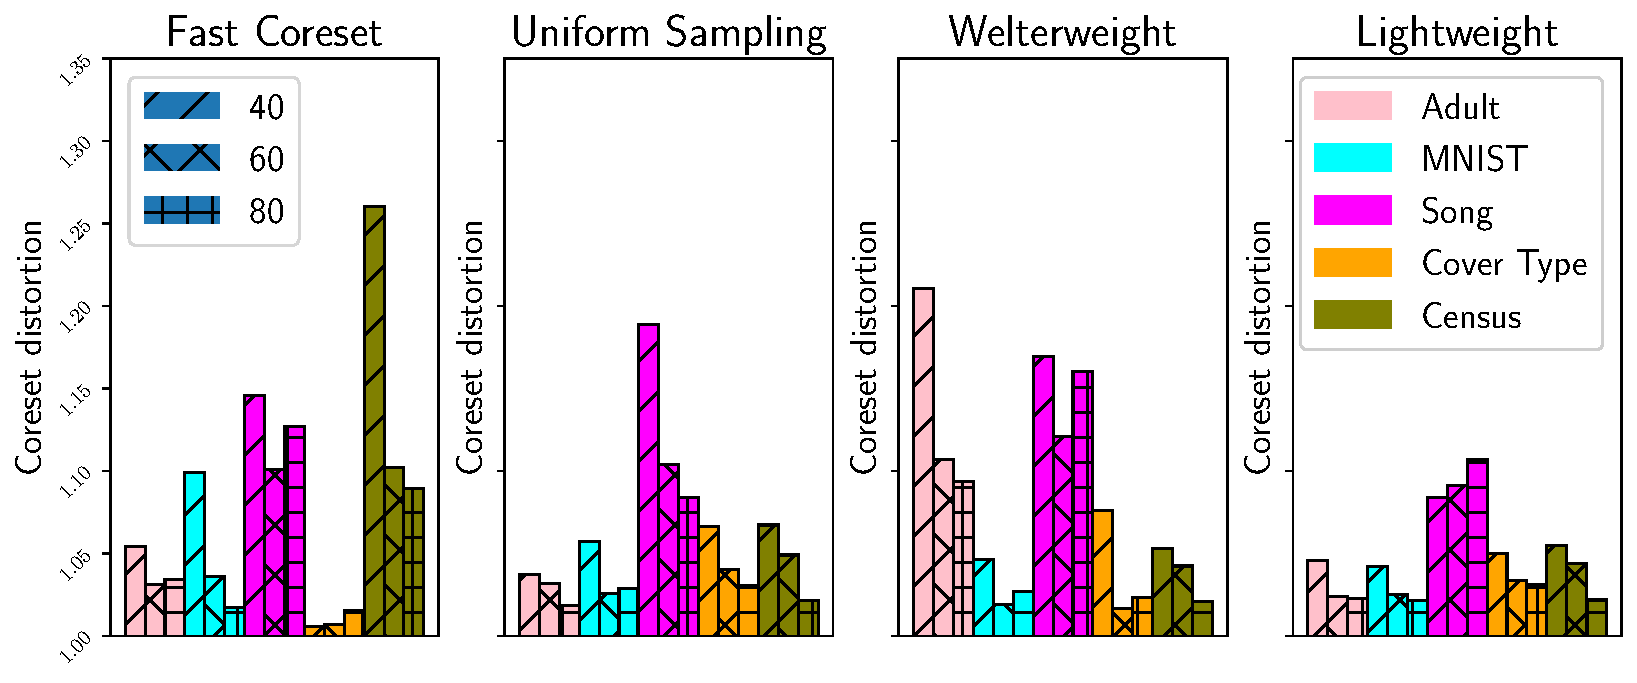
\includegraphics[width=\linewidth]{images/distortion_real_data} \\
    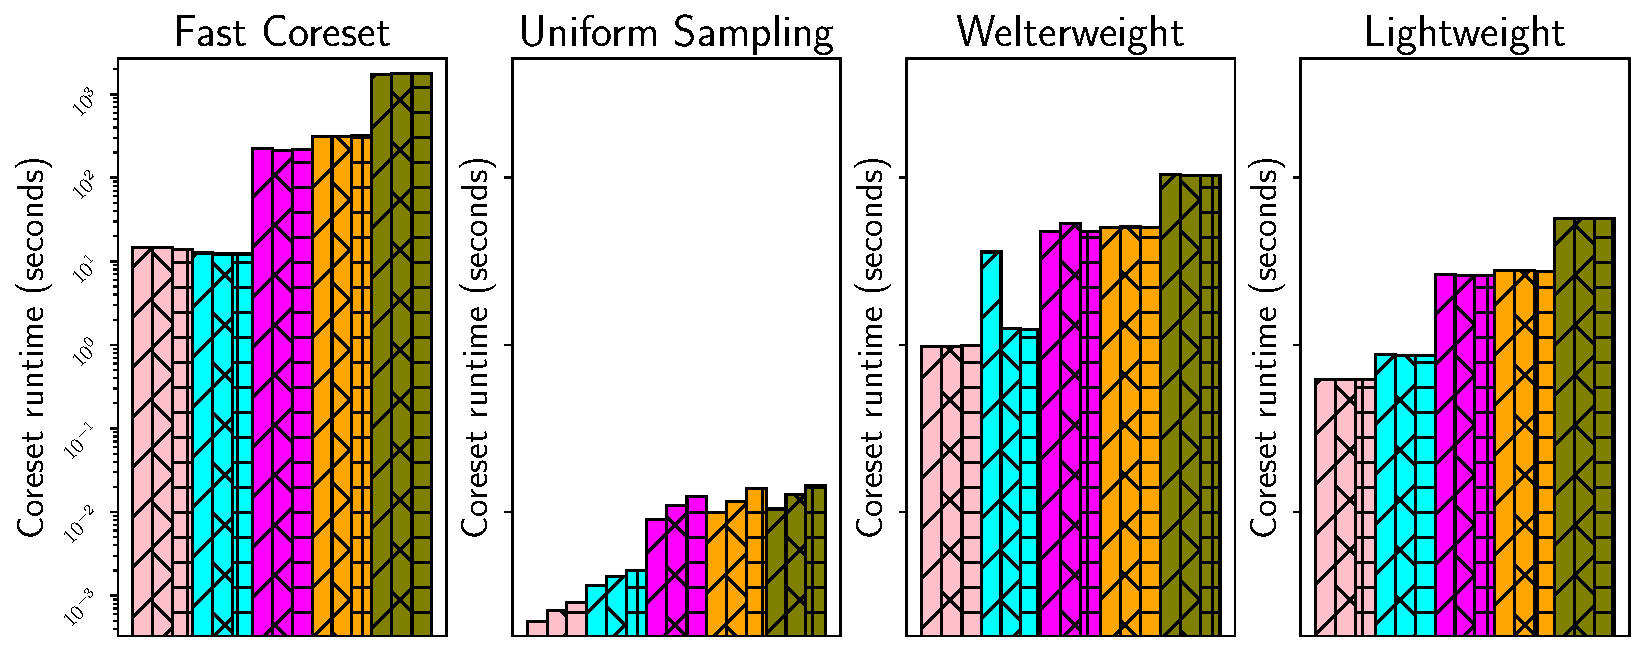
\includegraphics[width=\linewidth]{images/runtime_real_data}
\end{tabular}

\caption{\emph{Top}: The effect of the $m$-scalar on coreset distortion for real-world datasets. This is a visualization of the data in
Table~\ref{tbl:distortion}.  \emph{Bottom}: The effect of the $m$-scalar on the algorithm runtime for real-world datasets. All values are the mean over 5 runs.
The three bars represent samples of size $m=40k, 60k, 80k$.}

\label{fig:coreset_size_on_quality}
\end{figure}


We now refer the reader to the remaining columns of Table~\ref{tbl:distortion} and Figure~\ref{fig:coreset_size_on_quality}, where we show the effect of coreset
size across datasets by sweeping over $m$-scalar values. Despite the suboptimal theoretical guarantees of the accelerated sampling methods, we see that they
obtain competitive distortions on the real-world datasets while running faster than Fast-Coresets in practice. We attribute this to the well-behaved nature of
the real-world datasets, where they have few outliers and consistent class sizes.

To verify this, consider the results of these sampling strategies on the artificial datasets in Table~\ref{tbl:distortion} and
Figure~\ref{fig:coreset_size_on_quality}: as disparity in cluster sizes and distributions grows, the accelerated sampling methods have difficulty capturing all
of the outlying points in the dataset. Thus, Figure~\ref{fig:coreset_size_on_quality} shows a clear interplay between runtime and sample quality: \emph{the
faster the method, the more brittle its compression}.

\begin{figure*}
\label{fig:lightweight_breaks}
\centering
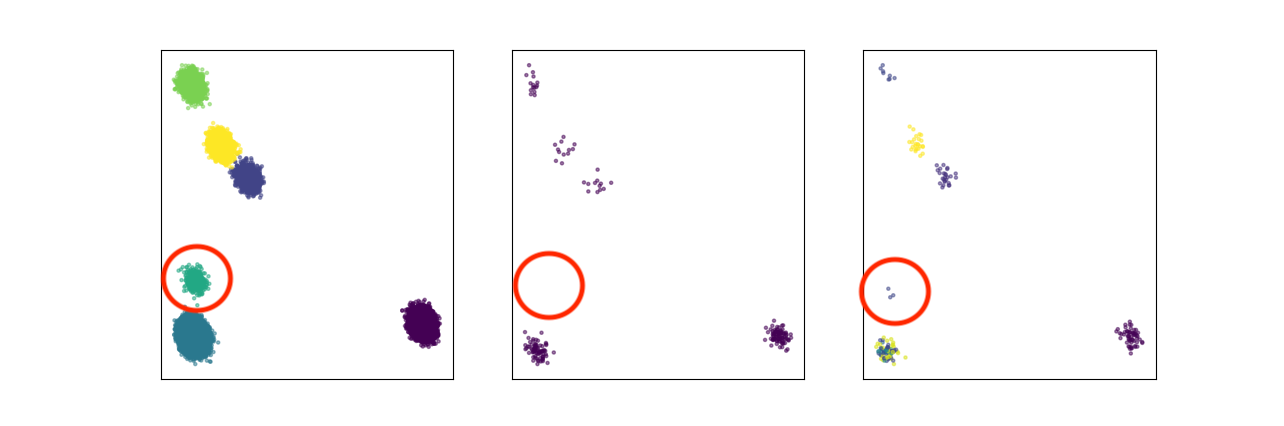
\includegraphics[width=.95\linewidth]{images/lightweight_breaks.png}
\caption{
The results of lightweight and fast-coreset constructions on a dataset of $n=100K$ points with clusters of varying size. Coresets have 200 points.
\emph{Left}: Original multivariate-Gaussian dataset. \emph{Middle}: Lightweight coresets fail to capture the cluster of $\sim$400 points.
\emph{Right}: The Fast-coreset construction runs in linear time but identifies all of the clusters.
}
\end{figure*}


While uniform sampling is expected to be brittle, it may be less obvious what causes light- and welterweight coresets to break. The explanation is simple for
lightweight coresets: they sample according to the $1$-means solution and are therefore biased towards points that are far from the mean. Thus, as a simple
counterexample, lightweight coresets are likely to miss a small cluster that is close to the center-of-mass of the dataset. This can be seen in
Figure~\ref{fig:lightweight_breaks}, where we show an example where the lightweight coreset construction fails on the Gaussian mixture dataset. Since the small
circled cluster is close to the center-of-mass of the dataset, it is missed when sampling according to distance from the mean.

Generalizing this reasoning also explains the brittleness of welterweight coresets when $j<k$. To see this, let $\calC_j$ be the approximation obtained during
welterweight coresets and observe that the sum of importance values of the points belonging to center $c_i \in \calC_j$ is \[ \sum_{p \in c_i} \left[
\dfrac{\cost(p, c_i)}{\cost(c_i, \calC_j)} + \dfrac{1}{|c_i|} \right] = \dfrac{\sum_{p \in c_i} \cost(p, c_i)}{\cost(c_i, \calC_j)} + 1 = 2.\] Thus, our
probability mass is distributed across the clusters that have been found in the approximate solution. Naturally, if $j < k$ and we missed a cluster from $\opt$,
there is some set of points that have not received an appropriate probability mass and may therefore be missed.

\begin{table}[htbp]
    \centering
    \small
    \begin{tabular}{lcccc}
        Algorithm & $\gamma = 0$ & $\gamma = 1$ & $\gamma = 3$ & $\gamma = 5$\\
        \hline
        \vspace*{-0.15cm}\\
        LW Coreset & 1.03 & 1.03 & 1.36 & 2.17\\
        $j=2$ & 1.04 & 1.04 & 1.04 & 1.92\\
        $j=\log k$ & 1.04 & 1.04 & 1.04 & 1.95\\
        $j=\sqrt{k}$ & 1.05 & 1.06 & 1.04 & 1.18\\
        Fast Coreset & 1.03 & 1.03 & 1.04 & 1.12\\
        \vspace*{-0.15cm}\\
    \end{tabular}
    \caption{The effect of $\gamma$ in the Gaussian mixture dataset on the coreset distortion. We report the means over 5 random dataset generations.
    Each generation had 50\,000 points in 50 dimensions, with 50 Gaussian clusters and coresets of size 4\,000. We set $k=100$.}
    \label{tbl:class-imbalance}
\end{table}



We evaluate the full extent of this relationship in Table~\ref{tbl:class-imbalance}, where we show the interplay between the welterweight coreset's $j$
parameter (number of centers in the approximate solution) and the Gaussian mixture dataset's $\gamma$ parameter (higher $\gamma$ leads to higher class
imbalance). We can consider this as answering the question ``How good must our approximate solution be before sensitivity sampling can handle class imbalance?''
To this end, all the methods have low distortion for small values of $\gamma$ but, as $\gamma$ grows, only Fast-Coresets (and, to a lesser extent,
welterweight coresets for larger values of $j$) are guaranteed to have low distortion.

\begin{figure}
    \centering
    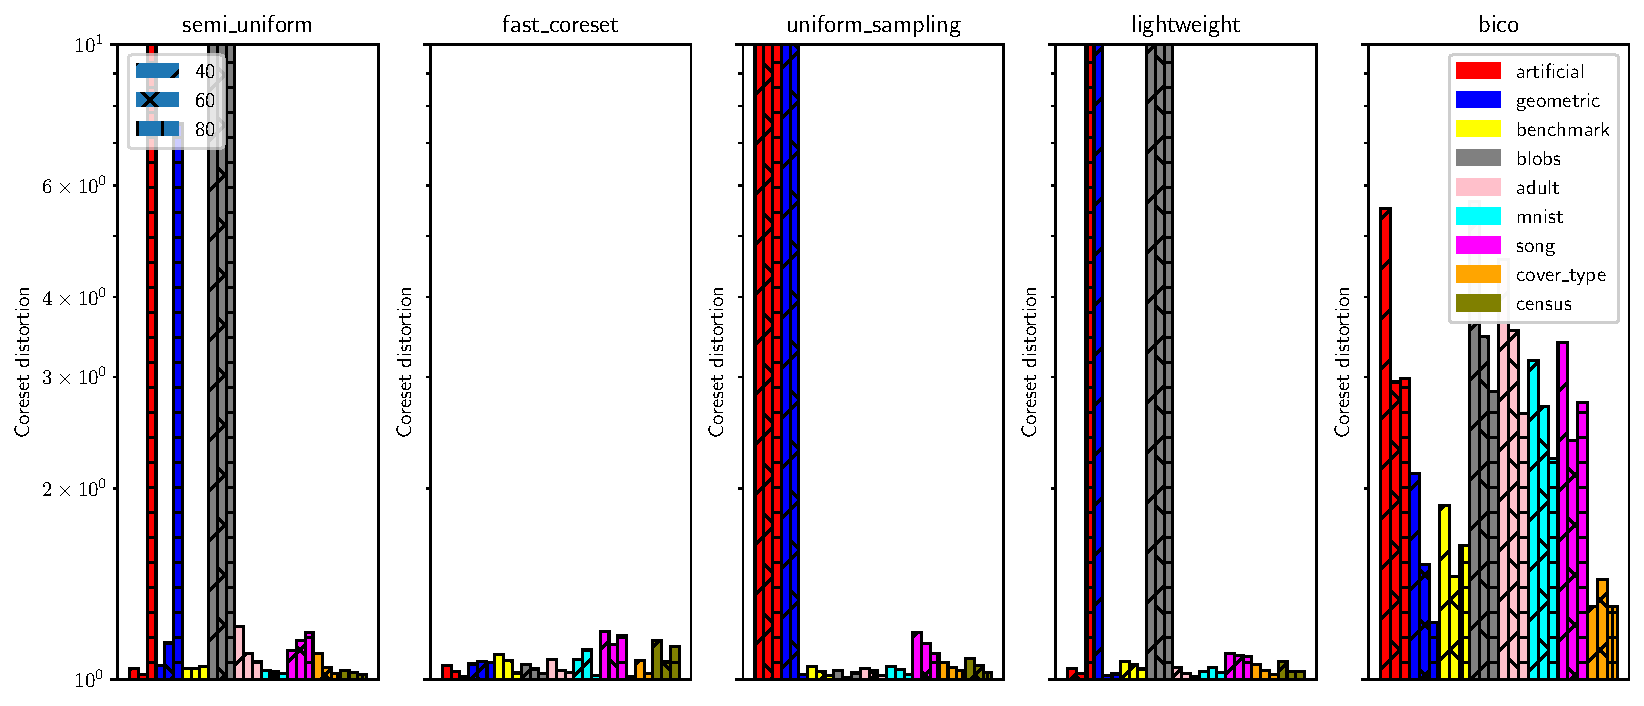
\includegraphics[width=\linewidth]{images/1/coreset_distortion-m_scalar_across_all_algorithms.pdf}
    \vspace*{-0.6cm}
    \caption{Sample coreset distortions under $k$-median for one run on each dataset. Bars within each dataset correspond to $m=40k, 60k, 80k$.}
    \label{subfig:kmedian_distortion}
\end{figure}
For completeness, we verify that these results also hold for the $k$-median task in Figure~\ref{subfig:kmedian_distortion}. There, we see that $k$-median
distortions across datasets are consistent with $k$-means distortions. We show one of five runs to emphasize the random nature of compression quality when using
various sampling schemas.

To round out the dataset analysis, we note that BICO performs consistently poorly on the coreset distortion metric\footnote{We do not include BICO in Figures
\ref{fig:coreset_size_on_quality}, \ref{subfig:kmedian_distortion}, \ref{fig:streaming_runtimes},  as it does not fall into the $\tilde{O}(nd)$ complexity class
and is only designed for $k$-means.}, as can be seen in Tables \ref{tbl:distortion} and \ref{tbl:composition}. We also point out that every sampling method
performs well on the benchmark dataset, which is designed to explicitly punish sensitivity sampling's reliance on the initial solution. Thus, we verify that
there is no worst-case setting that breaks sensitivity sampling.

We lastly show how well these compression schemas facilitate fast clustering on large datasets in Table~\ref{tbl:lloyds}. Consider that a large
coreset-distortion means that the centers obtained on the coreset poorly represent the full dataset. However, among sampling methods with small distortion, it
may be the case that one consistently leads to the `best' solutions. To test this, we compare the solution quality across all fast methods on the real-world
datasets, where coreset distortions are consistent. Indeed, Table~\ref{tbl:lloyds} shows that no sampling method leads to solutions with consistently minimal
costs.

\subsection{Streaming Setting}
\label{ssec:streaming}

\begin{figure}
    \centering
    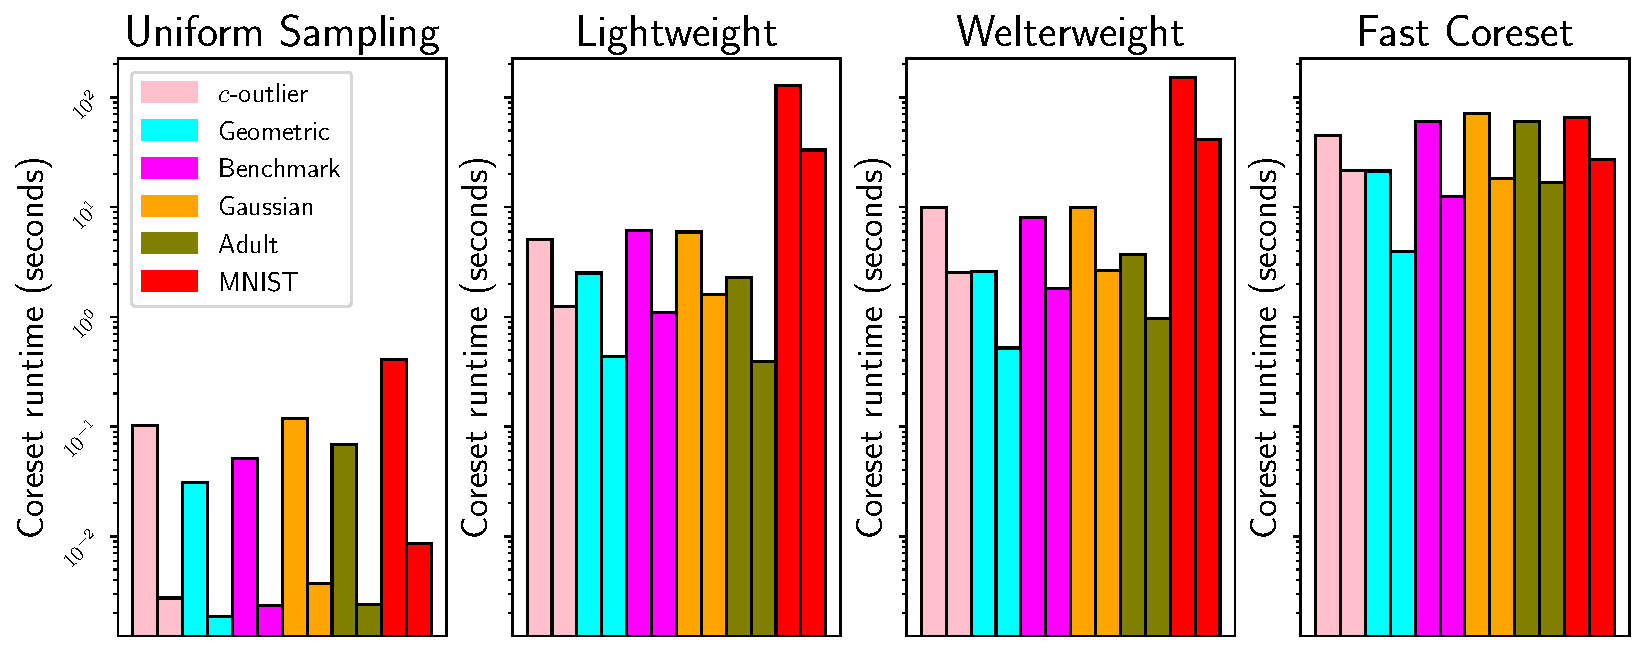
\includegraphics[width=.95\linewidth]{images/2/coreset_runtime-composition.pdf}
    \caption{Mean runtime over three runs in the streaming and non-streaming settings. Bars are [Streaming, Non-Streaming]; y-axis is log-scale.}
    \label{fig:coreset_size_on_sens_quality}
\end{figure}


One of the most common use-cases for big-data algorithms is the streaming setting, where one receives input in batches and must maintain a compression that is
representative of the dataset. Although there is a wealth of sampling and coreset methods in the streaming paradigm, we require consistency across algorithms
and therefore assume a black-box sampling procedure. Since the coreset property is preserved under composition, we utilize the merge-\&-reduce strategy
originally proposed by \cite{BS80} and first applied to maintaining clustering coresets in stream by \cite{HaM04}. The idea is to first partition the input into
$b$ blocks and then perform sampling and composition along them until a single compression is obtained. Specifically, we start by obtaining a coreset on each
block. Then, combining samples using a complete binary tree, we (1) recursively re-sample from the children until there is at least one coreset for each
level\footnote{If there are $b=8$ blocks, then there would be coresets corresponding to blocks $[[1], [2], [3, 4], [5, 6, 7, 8]]$} in the tree and then (2)
concatenate these samples and obtain one final coreset from the composition. Since we are composing coresets from coresets, the errors stack and, in theory, we
should require more samples to obtain a similar accuracy.

Despite this, we see the opposite result for many of our sampling strategies. Surprisingly, Table~\ref{tbl:composition} and Figure~\ref{fig:streaming_runtimes}
show that the accelerated sampling methods all perform \emph{better} under composition on the artificial datasets and do not suffer significant drops in
accuracy, variance or runtime on the real datasets. Although inconsistent with the prevailing intuition, we must therefore conclude that the accelerated
sampling methods are \emph{more} feasible in the streaming setting.  We suspect that this is due to the non-uniformity imposed by the merge-\&-reduce algorithm.
To see this, consider uniform sampling on the $c$-outlier dataset during the final step of the composition, where we are composing the samples corresponding to
each layer of the tree. Assume first that our outlier points happened to fall in the first block. Then we have taken a sample of size $m$ from this block and
immediately use this for the final composition. Thus, in this case the outliers are \emph{more} likely to be in our final sample than in the non-streaming
setting. In the alternate setting where the outliers are less likely, our expected error is already high and missing the outlier `more' cannot worsen our
expected error. 
